\documentclass[tikz,border=6pt]{standalone}
\usepackage{amsmath}
\begin{document}
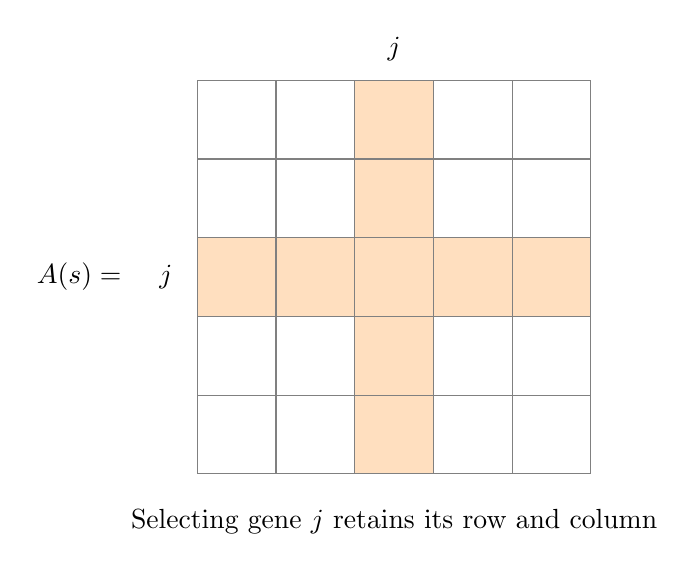
\begin{tikzpicture}
  \fill[orange!25] (0,2) rectangle (5,3);
  \fill[orange!25] (2,0) rectangle (3,5);
  \draw[step=1,gray] (0,0) grid (5,5);
  \node at (2.5,5.4) {$j$};
  \node at (-0.4,2.5) {$j$};
  \node at (-1.5,2.5) {$A(s)=$};
  \node at (2.5,-0.6) {Selecting gene $j$ retains its row and column};
\end{tikzpicture}
\end{document}
